\documentclass[a4paper, 12pt]{article}

\usepackage{fullpage}
\usepackage{amsmath,amsfonts,amssymb, amsthm, graphicx}
\usepackage{xcolor}

\usepackage{enumitem}
\setlist[1]{topsep=3pt,itemsep=3pt,parsep=3pt}

\usepackage{algorithm}
\usepackage{algpseudocode}
\algtext*{EndWhile}
\algtext*{EndIf}
\algtext*{EndFor}

\usepackage{url}
\usepackage{xspace}

\newcommand{\homework}[2]{
	\thispagestyle{plain}
	\setcounter{page}{1}
	\noindent
	\begin{center}
		\framebox{
			\vbox{\vspace{2mm}
				\hbox to 6.28in { {CSE 431/531: Algorithm Analysis and Design
						\hfill Fall 2021} }
				\vspace{4mm}
				\hbox to 6.28in { {\Large \bf \hfill Homework #1 \ifdefined\sol Solutions\fi \hfill} }
				\vspace{2mm}
				\hbox to 6.28in { {\it Instructor: Shi Li} \hfill {\bf Deadline: #2} }
				\vspace{2mm}}
		}\medskip
		
		Your Name: \underline{\ \ \ \ \ \ \ \ \ \ \ \ \ \ \ \ \ \ \ \ \ \ \ \ \ \ \ \ \ \ \ \ \ } \qquad Your Student ID: \underline{\ \ \ \ \ \ \ \ \ \ \ \ \ \ \ \ \ \ \ \ \ \ \ \ }
	\end{center}
}

\DeclareMathOperator{\E}{\mathbb{E}}
\DeclareMathOperator{\union}{\bigcup}

\newcommand\floor[1]{\left\lfloor#1\right\rfloor}
\newcommand\ceil[1]{\left\lceil#1\right\rceil}
\newcommand\set[1]{\left\{#1\right\}}

\newcommand{\R}{{\mathbb{R}}}
\newcommand{\Z}{{\mathbb{Z}}}
\newcommand{\C}{{\mathbb{C}}}
\newcommand{\Q}{{\mathbb{Q}}}

\renewcommand{\P}{{\textbf{P}}\xspace}
\newcommand{\NP}{{\textbf{NP}}\xspace}
\newcommand{\poly}{{\mathrm{poly}}}


\begin{document}
	
	\homework{1}{9/28/2021}

	\begin{table}[h]
		\centering
		\begin{tabular}{|c|c|c|c|c|}
			\hline
			Problems &1&2&3& Total \\ \hline
			Max. Score & 20  & 30 & 30 & 80 \\ \hline
			Your Score & &  & & \\ \hline
		\end{tabular}
	\end{table}
	\bigskip
	
\paragraph{Problem 1.} 		For each pair of functions $f$ and $g$ in the following table, indicate whether $f = O(g), f = \Omega(g)$ and $f = \Theta(g)$ respectively.  Then prove $\ceil{10 n^{1.9}} = O(n^2)$.
		\begin{table}[h]
			\centering 
			\renewcommand{\arraystretch}{1.5}
			\begin{tabular}{|c|c||c|c|c|}
				\hline
				$f(n)$ & $g(n)$ & $O$ & $\Omega$ & $\Theta$\\ \hline
				$n^2 - 3n + 10$ &  $n $ & & & \\ \hline
				$\log_{3} n$ & $10\log_2 (n^3)$  & & & \\ \hline
				$10n^2-  n$ &  $n^2 \log n$ & & & \\ \hline
			\end{tabular}
		\end{table}
		
%\paragraph{Problem 3.} Consider the Euclidean algorithm for computing the greatest common divisor of two integers $a, b > 0$: 
%		\begin{algorithm}[H]
%			\caption{Euclid$(a, b)$}
%			\begin{algorithmic}[1]
%				\While{$b > 0$ }
%					\State$t \leftarrow b$;
%					\State$b \leftarrow a\text{ mod } b$;
%					\State$a \leftarrow t$;
%					\State\Return $a$
%				\EndWhile
%			\end{algorithmic}
%		\end{algorithm}
%		
%		Prove that the algorithm terminates in $O(\lg a)$ iterations. 
	
\paragraph{Problem 2.}

		Given a \emph{sorted} array $A$ of size $n$, design an algorithm to check if there are two numbers in the array whose sum is $0$.   That is, decide whether there are two indices $i, j \in \{1, 2, 3\cdots, n\}$ such that $A[i] + A[j] = 0$. (The two indices can be the same; thus if the array contains the number 0, we should output ``yes''.) 
		
		Example: if the input is $(-8, -5, -2, 1, 4, 6, 8, 9)$, then the output is ``yes'' since $(-8) + 8 = 0$.  If the input is $(-8, -5, -2, 1, 4, 6, 7, 9)$, then the output is ``no''. 
		Design an $O(n)$-time algorithm for the problem.\smallskip

\noindent\begin{minipage}{0.6\textwidth}
		\paragraph{Problem 3.} 
		A cycle in a \emph{directed} graph $G = (V, E)$ is a sequence of $t \geq 2$ \emph{different} vertices $v_1, v_2, \cdots, v_t$ such that $(v_i, v_{i+1}) \in E$ for every $i = 1, 2, \cdots, t-1$ and $(v_t, v_1) \in E$. See Figure 1 for an example. Given the linked-list representation of a directed graph $G = (V, E)$ with $n = |V|$ and $m = |E|$, design an $O(n + m)$-time algorithm to decide if $G$ contains a cycle or not; if it contains a cycle, output one (you only need to output one cycle).
		
		You can use topological ordering as a sub-procedure. If you do, it is not necessary to write down the whole pseudo-code for the procedure. 
	\end{minipage}
	\hfill
	\begin{minipage}{0.3\textwidth}
		\begin{figure}[H]
			\centering
			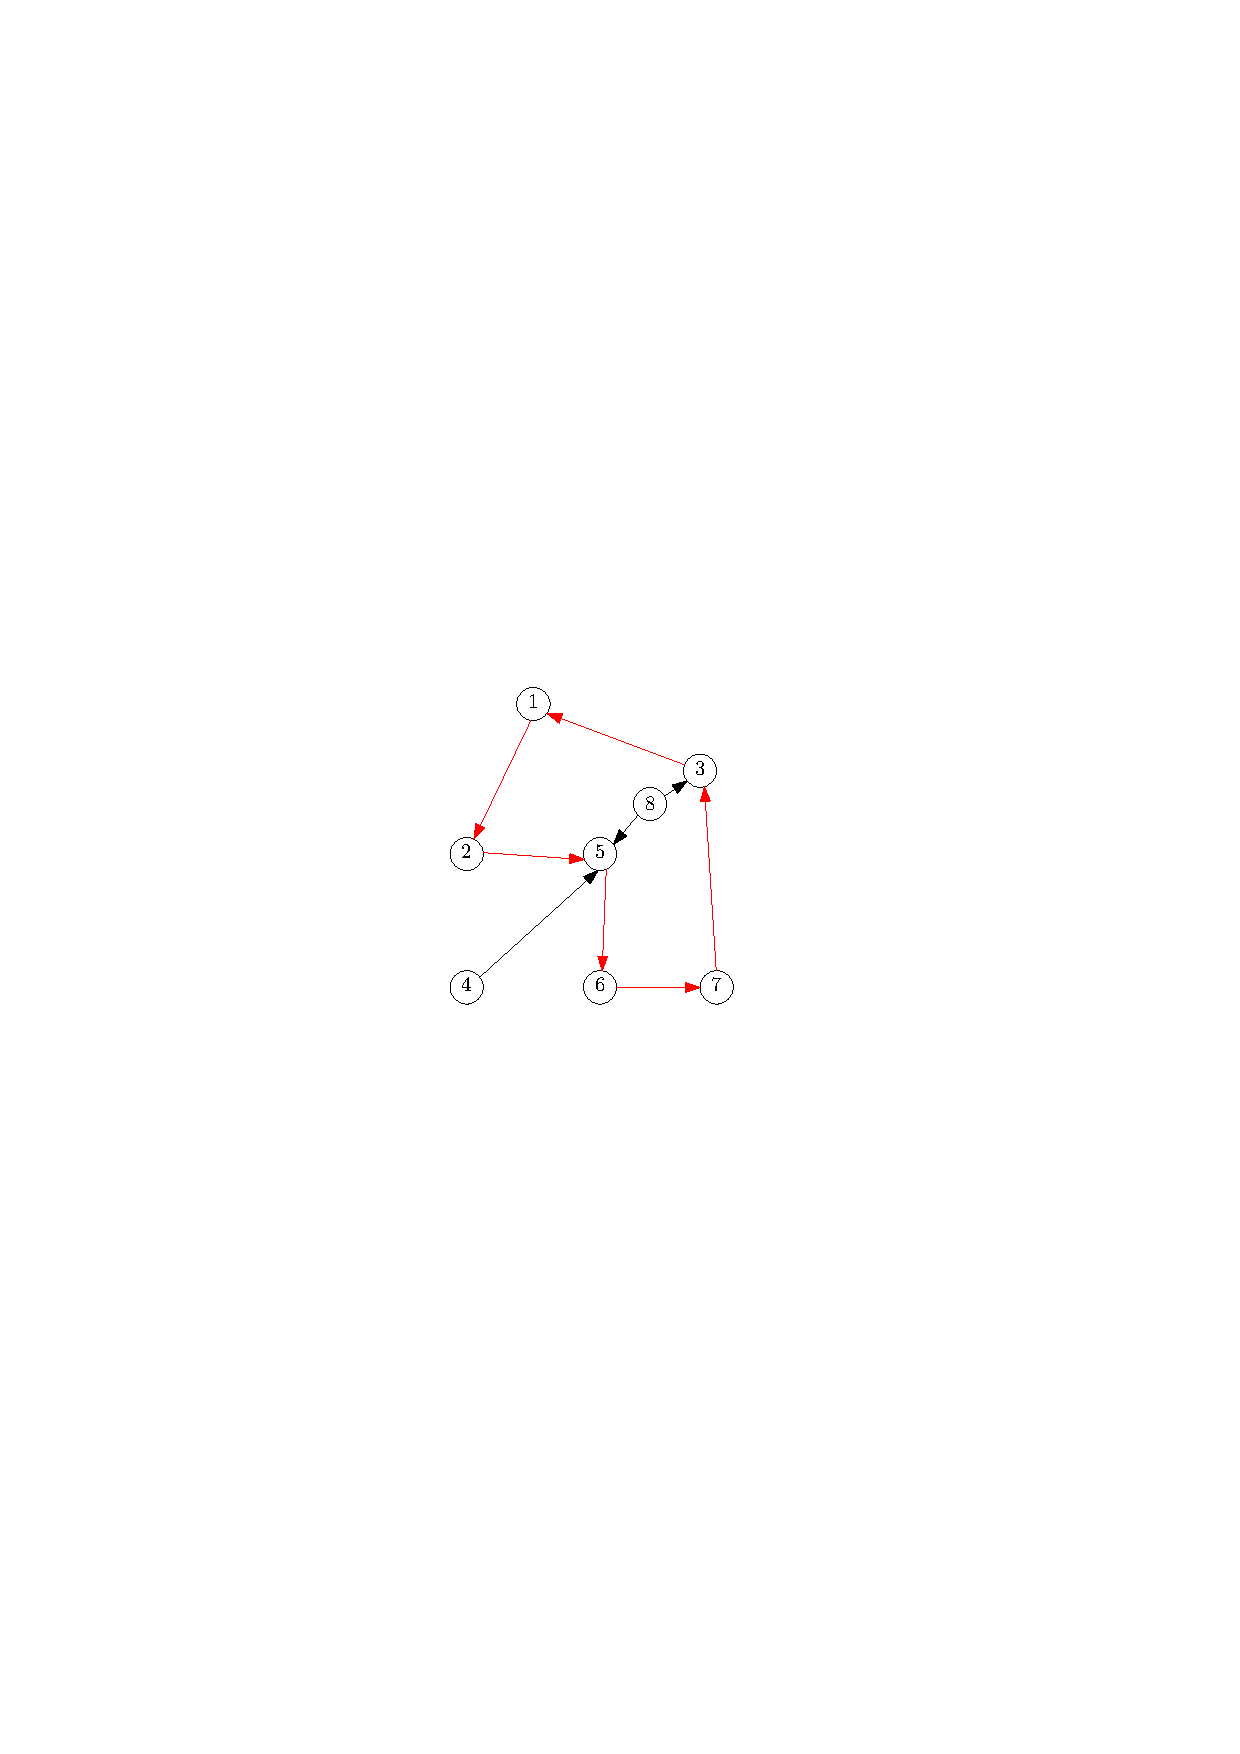
\includegraphics[width=0.7\textwidth]{cycle}
			\caption{A cycle (denoted by red edges) in a directed graph.}
		\end{figure}
	\end{minipage}
\end{document}